\chapter{Reducing Object Bloat}

In many applications, the heap is filled mostly with instances of just a few
important classes.  You can increase scalability significantly by making these
classes as compact as possible. This chapter describes field usage
patterns that can be easily optimized for space, for example, fields that are
rarely needed, constant fields, and dependent fields. Simple refactoring of
these kinds of fields can sometimes result in big wins.
 

\section{Rarely Used Fields}

Chapter~\ref{chapter:delegation} presents examples where delegating fields
to another class increases memory cost. However, sometimes delegation can
actually save memory, if you don't have to allocate the delegated object all the
time.

As an example, consider an on-line store with millions of products. 
Most of the products are supplied by the parent company, but
sometimes the store sells products from another company:
\begin{shortlisting} 
class Product {
	String sku;
	String name;
	..
	String alternateSupplierName;
	String alternateSupplierAddress;
	String alternateSupplierSku;
}
\end{shortlisting}
When there is no alternate supplier, the last three fields
are never used. By moving these fields to a separate side class, you can
 save memory, provided the side object is allocated only when
it is actually needed. This is called \emph{lazy allocation}.

\begin{shortlisting} 
class Product {
	String sku;
	String name;
	.. 
	Supplier alternateSupplier;
}

class Supplier {
	String supplierName;
	String supplierAddress;
	String sku;
}
\end{shortlisting}
For products with no alternate supplier, eight bytes are saved per product,
since three fields are replaced by one. Of course, products with an alternate
supplier pay a delegation cost, including an extra pointer and object header.
The question is how much total memory is actually saved, if any? The answer
depends on the percentage of products that have an alternate supplier needing a
side object, which we'll call the \emph{fill rate}.

Figure~\ref{fig:fill-rate} shows the memory saved for different
fill rates, assuming three fields (12 bytes) are delegated. The most memory that can
be saved is 66\%, when the fill rate is
0\%. When the fill rate is 10\%, 50\% of memory is saved. 
When the fill rate is over 40\%, the memory saved is
negative, that is, memory is wasted. The lesson here is that if you aren't sure
what the fill rate is, then using delegation to save memory may end up
backfiring.
\begin{figure}
  \centering
 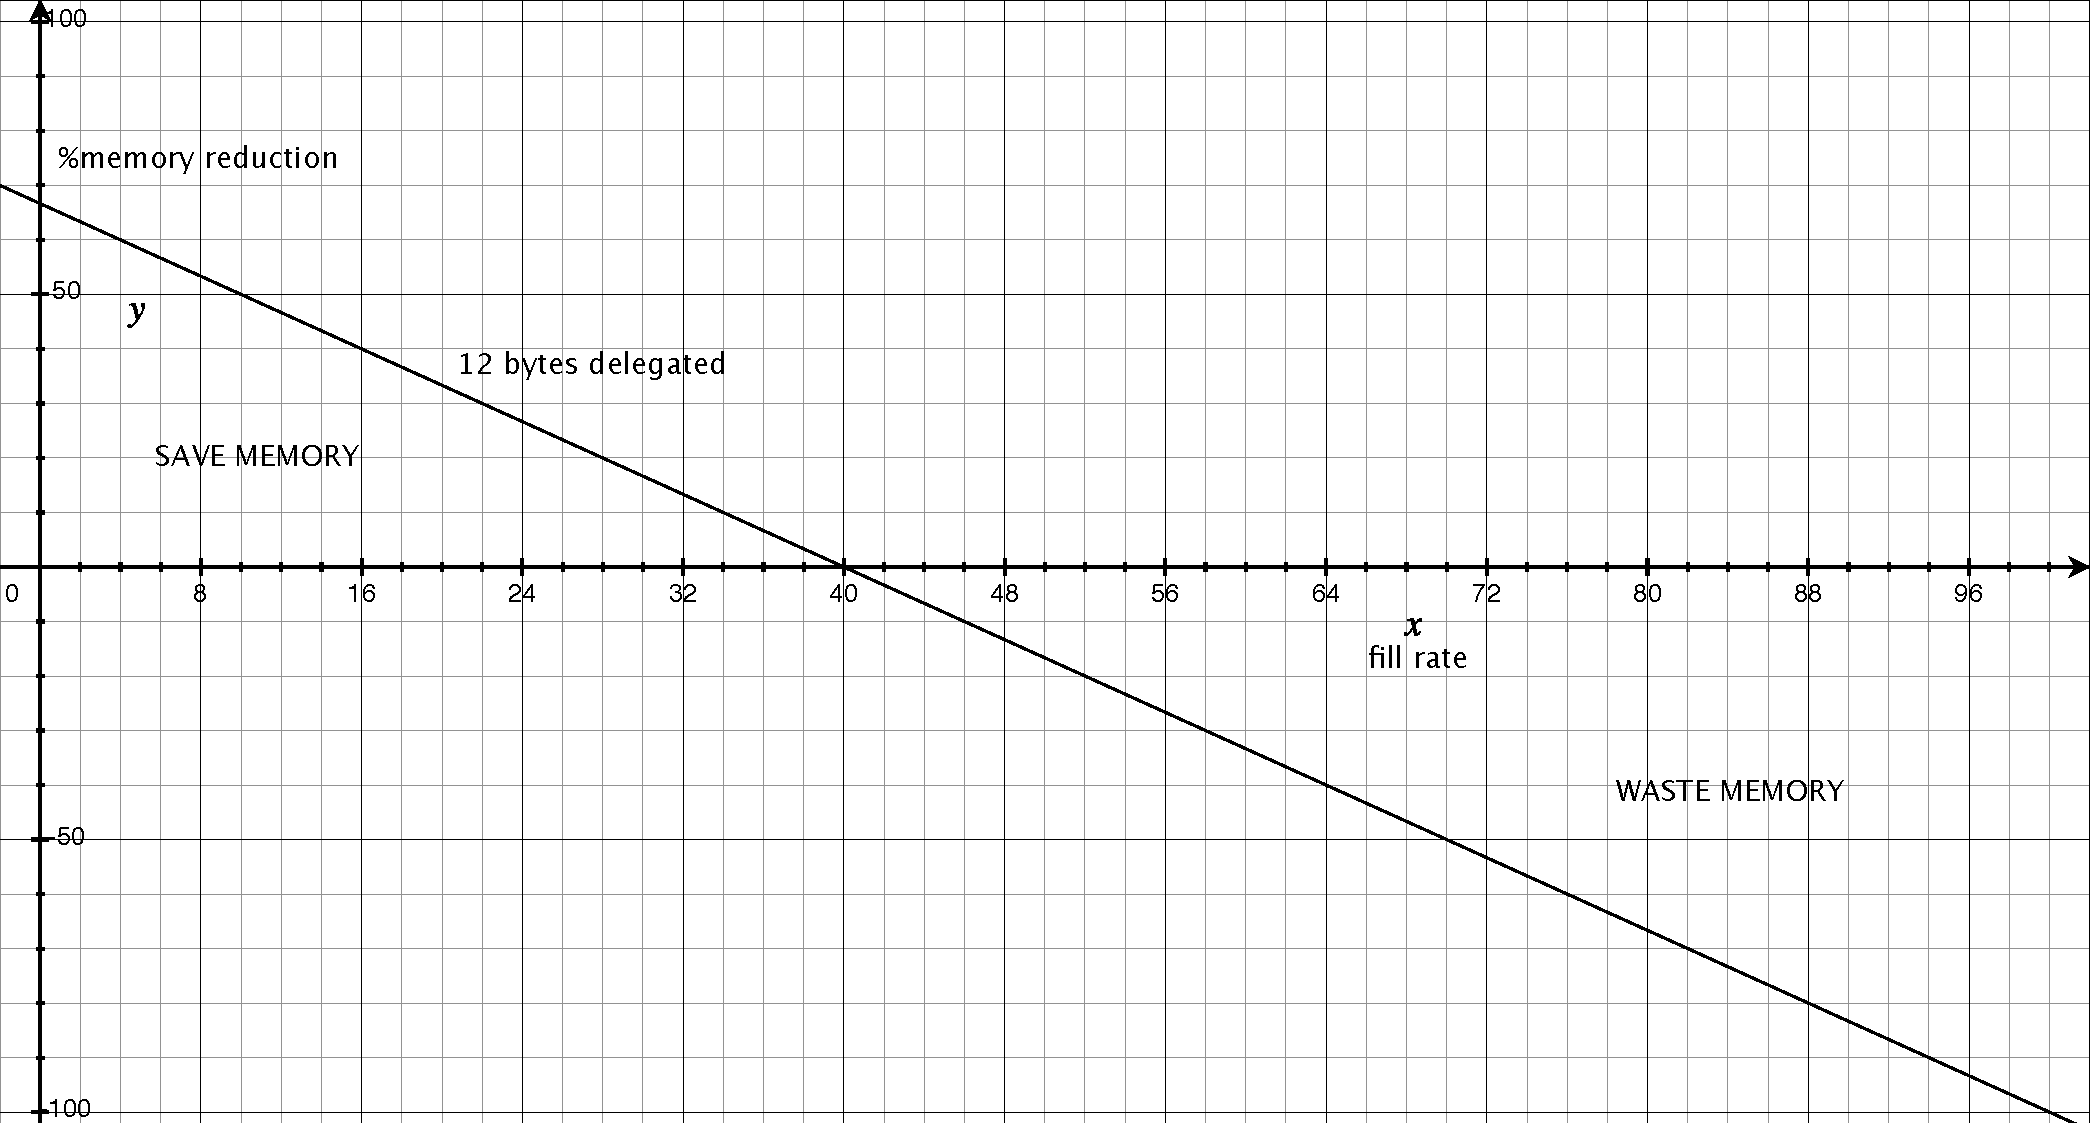
\includegraphics[width=.90\textwidth]{part2/Figures/chapter4/12-byte-graph.pdf}
 % 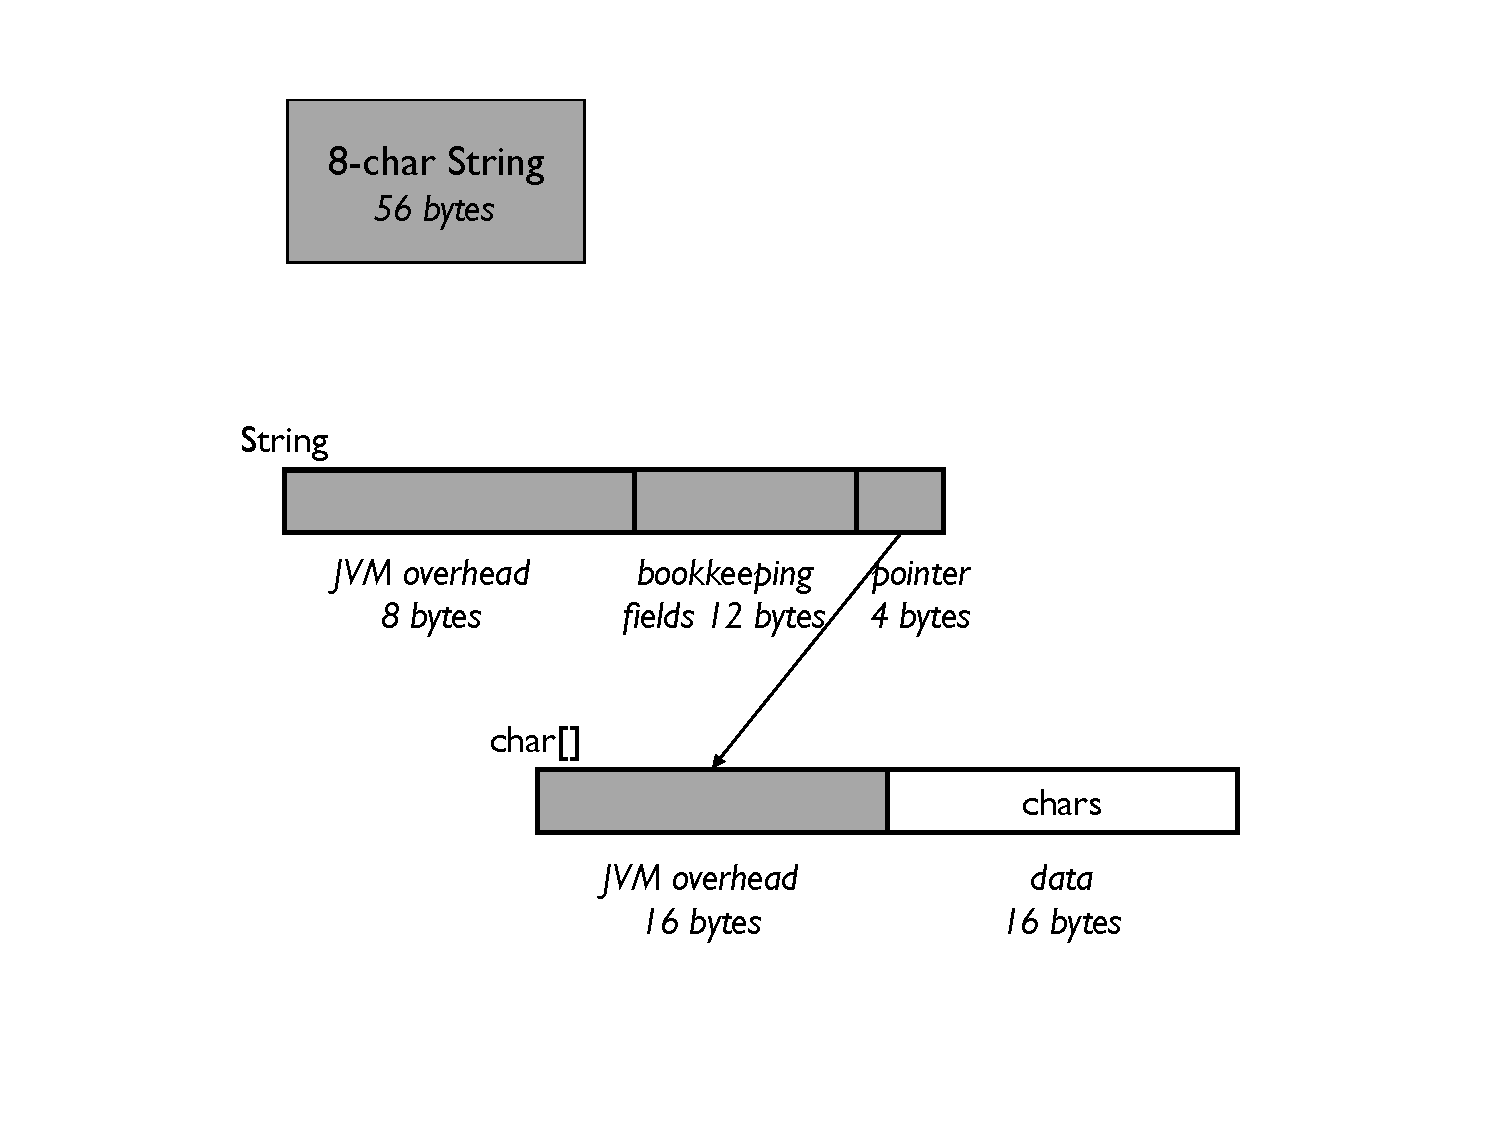
\includegraphics{eight-char-string}
  \caption{This plot shows how much memory is saved or wasted by delegating 12
  bytes of memory to a side object. The x-axis is the fill rate, and the
  y-axis is the percent of memory saved.}
  \label{fig:fill-rate}
\end{figure}
In addition to the fill rate, the memory savings also depends on the
number of fields delegated. The more bytes delegated, the larger the memory
savings, assuming the same fill rate. Figure~\ref{fig:rarely-used} shows the memory
saved for different fill rates and different delegated-field sizes. Each
line represents a different delegated-field size. The bottom-most line
represents a delegated field size of 16 bytes, the next line represents 32 bytes, the next
represents 48 bytes, and so on, up to 144 bytes. As the delegation size
increases, you can worry less about the fill rate. For example, if 32 bytes
are delegated, there is almost 90\% savings with a low fill rate, and some
memory savings with a fill rate up to 70\%. As the delegation size increases, 
the lines start to converge, since the fixed delegation cost becomes relatively
less important.
\begin{figure}
  \centering
 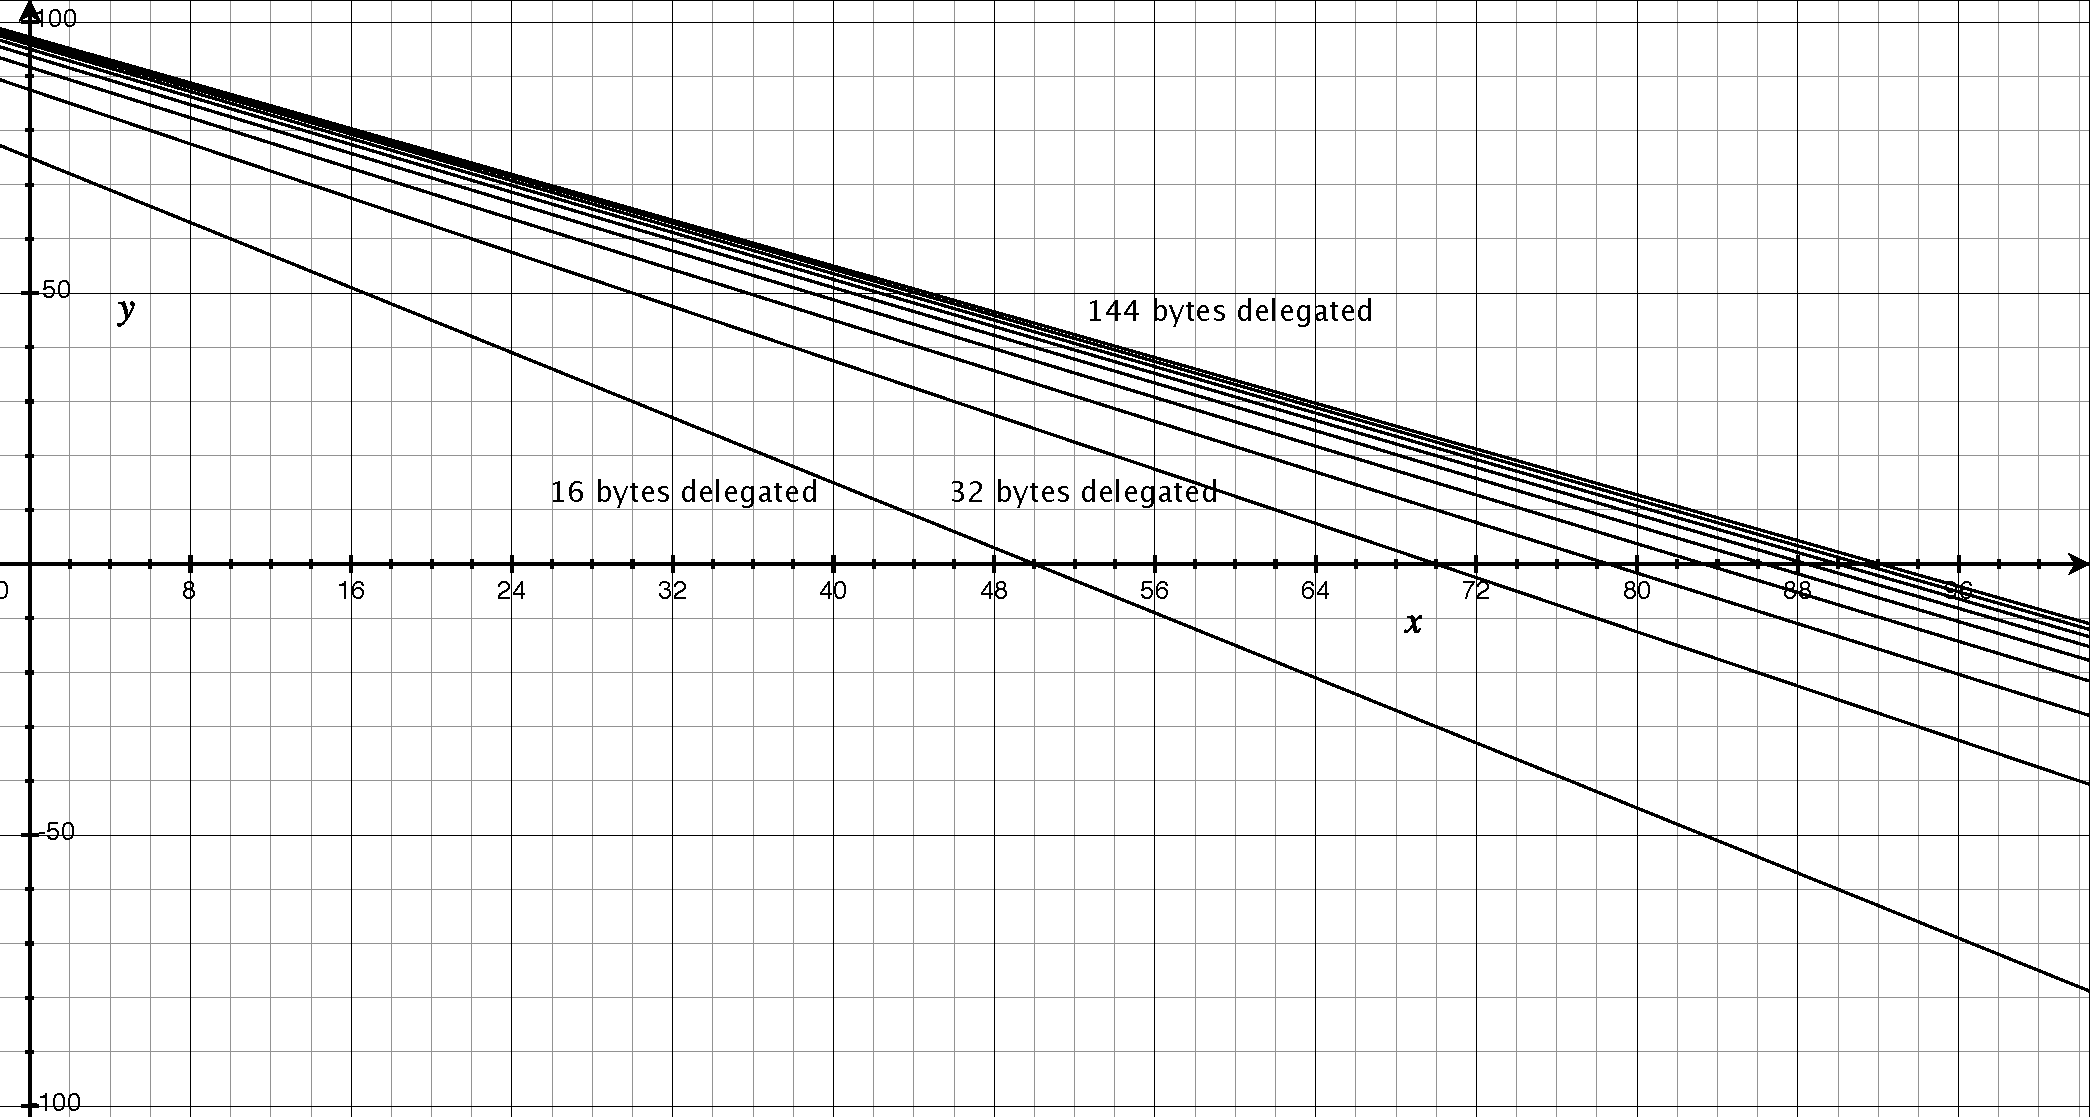
\includegraphics[width=.90\textwidth]{part2/Figures/chapter4/rarely-used.pdf}
 % 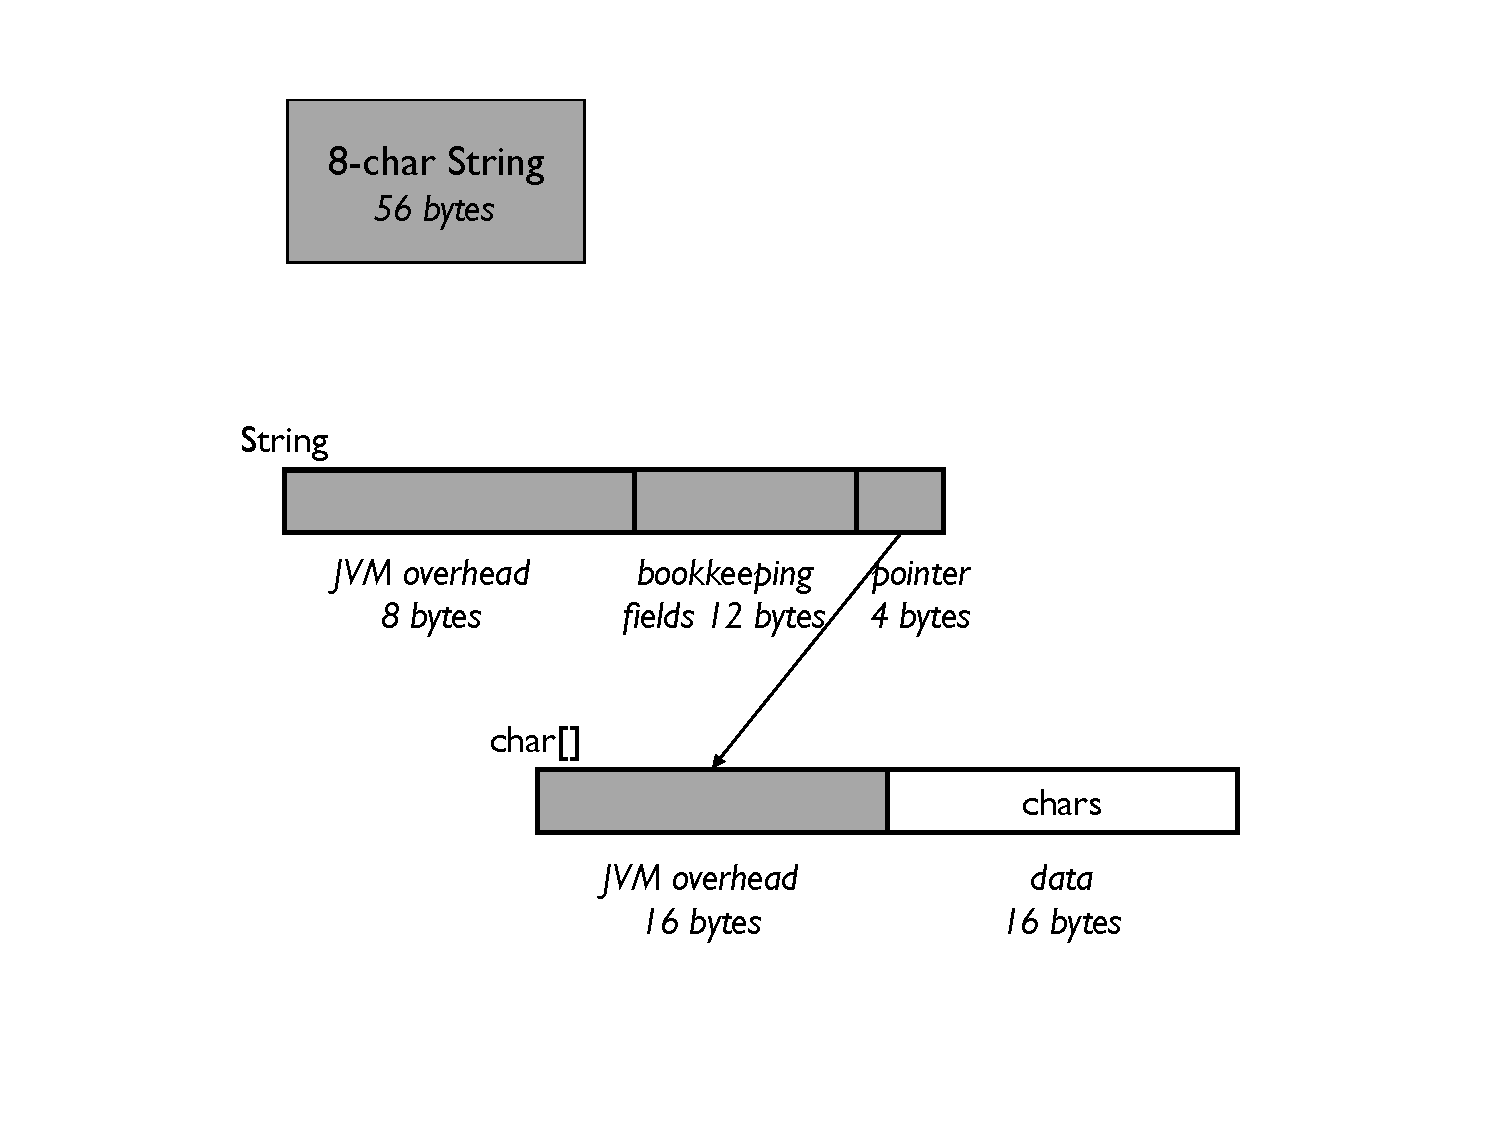
\includegraphics{eight-char-string}
  \caption{This plot shows how much memory is saved or wasted for different
  delegate field sizes. The x-axis is the fill rate, and the y-axis is the
  percent of memory saved. Each line represents a different delegated size,
  starting from 16 bytes, going up to 144 bytes by increments of 16 bytes.}
  \label{fig:rarely-used}
\end{figure}

\callout{callout:rarely-used}{Delegation Cost Calculation}{
\index{Delegation Cost Calculation}
Assume the cost of a pointer is 4 bytes, and the cost of an object header is 8
bytes. Let $B$ = the size in bytes of a set of fields being delegated, and
$F$ = the fill rate. Then the memory cost of the delegated
implementation per object is:
\begin{eqnarray}
D &=& F(B+8)+4 \nonumber
\end{eqnarray}
Note that every object pays a 4 byte pointer cost, and only $F$ of
the objects pay for the side object. The proportional improvement is:
\begin{eqnarray}
\frac{(B-D)}{B} &=& 1 - \frac{D}{B} \nonumber \\
&=& 1 - \frac{(F(B+8)+4)}{B} \nonumber.
\end{eqnarray}
The following equation can be used to obtain the plots in
Figures~\ref{fig:fill-rate} and~\ref{fig:rarely-used}, for different values of
$B$:
\begin{eqnarray}
y &=& 100*(1 - \frac{\frac{x}{100}(B+8)+4}{B})
\end{eqnarray}
} 
A common error is to delegate rarely-used fields to a side class, but forget to
allocate it only when needed, that is, always allocate a side object. 
In this case, instead of saving memory, you pay the full cost of delegation as well as 
the cost of unused fields. 
Lazy allocation
can be error-prone, since it may require testing whether the object exists at
every use. This complexity has to be weighed against potential memory
savings.

\section{Constant Fields}

Recognizing when a field can be declared \code{static} is a simple way to
save memory. Programmers usually remember to make constants like \emph{pi} 
static. There are other situations that are a bit more subtle, for example,
when a field is looked at out of context.

Returning to the product example, suppose that each product has a field
\code{catalog} that points to a store catelog.
If you know that there is always just one store catalog, then the field
\code{catalog} can be turned into a static, saving 4 bytes per product.

As a more elaborate example, suppose that every product belongs to a
category such as books, music, clothes, toys, etc, and 
 has a field pointing to a \class{Category} object.
These fields are clearly not the same across all products. However, suppose we
define
subclasses \class{Book}, \class{Music}, \class{Clothing} of \class{Product}, 
where all instances of a subclass belong to the same category.  
Now the \code{category} field is the same for products in each subclass,
so it can be made static:

\begin{shortlisting} 
class Book extends Product {
	static Category bookCategory; 	// points to the book category object  
	..
}

class Music extends Product {
	static Category musicCategory;  // points to the music category object
	..
}

class Clothing extends Product {
	static Category clothingCategory;  // points to the clothing category object
	.. 
}
\end{shortlisting}

Knowing the context of how objects are created and used, and how they relate to
other objects, is helpful in making these kinds of memory optimizations.


\section{Mutually Exclusive Fields}

Sometimes a class has fields that are never used at the same time, and possibly
they can share the same space. Unfortunately, Java does not have anything like
a union type, so sharing space is often not possible. However, there are some
limited opportunities to take advantage of mutually exclusive fields to save
memory.

The next problem we found is that in some cases, you
 still needed this thing, even when it was rightfully being lazily allocated, and so it had 5 bookkeeping fields, and we took a 
look at those fields, and we realized they were never all used at the same time. They each 
covered different cases, and there were various combinations, and you never needed all of them. 
You usually only needed 2 or 3 of them at a time. So I believe what they did, or what they were 
planning to do, is combine some of those fields, and basically loosen the typing a bit, and use 
casts, so share one field, get Capital Object, and then the accessor to it, recast it to it�s 
actual use case. So that�s sort of like a poor man�s loosely typed union, and so if Java had 
type safe unions, you wouldn�t need that, and the compiler could do a better job with that too. 


\section{Redundant Fields}

A lot of the data type modeling patterns we talked about were either delation or things 
having overhead fields, and in some cases we had too much data also.  I want to follow up on a 
few patterns in that area.  Having more data than you really need. In some sense that�s another 
kind of overhead.  

(two types � can be computed rather than stored, or not.)

Another case they had, they had one or two of those bookkeeping fields were stored computations, 
they were caching things, so they were actually leaving pointer space to cache something, and 
then the cache of it was another side object holding onto stuff, and in some cases that was 
a collection. And it turns out that that was rarely needed. So I don�t know if they actually 
fixed that, but I believe they did. So again, these are very typical of the kinds of problems you 
see. You don�t usually see one big problem making an instance size big. You usually see a 
smattering of all these little kinds of things, and they add up.

The other thing is, and I just have one example of it here, but there are many more in these 
types. See this typeID, then string of type, so each of these has a type, and they are storing 
it, and they are storing the formatted version of it also, and so they are allocating basically 
2 fields for every every logical field here. An int and a pointer. In the next session we will 
look at other implications of that. This is something they did over and over again, like this 
in the electronic address, the physical address. A lot of these bytes have to do with the fact 
that they were storing these things twice. So just the field cost of that was huge. 

So the first problem is hard to fix, in that there is a refactoring. The second problem is easy, 
just not storing and recomputing it. The second problem is easy, just not storing and recomputing 
it. (In this case, the database stored both fields as well.)

So what they were doing there, was they were saving both a binary version, and an ASCII 
formatted version of the same field, and they were doing that for a lot of fields. 
And since this was a delegated design, this was multiplied everywhere. So it really added up.  
We looked at the field cost, last time, in the actual objects making up the profile, 
but the other thing that is super common is that they were pointing to Strings, 
actually storing the data, and the actual cost of the Strings was pretty high. 
So the na�ve view, especially if you are used to languages like C, is that, what�s a couple of 
characters?  I�ll just store �Y� or �N�, what�s the big deal of storing one or two characters. 
But as we saw, looking inside the string, the health ratio for something like Y or an N, 
a single character, is 48:1. It takes about 44 bytes to store that string, plus the pointer to 
et there. In some cases these were either constant, or there were things that have just a 
few values. I think it just had three values, where every single record had both an int, or a 
short, and had the pointer to a string, which said Y or N.  This is a super common problem, 
is duplicating data that has a high overhead in its representation. That combination is all over 
the place, and Strings is the big culprit. They had another field like that. 
It was a policy threshold, and it was a constant every single record had this
10\% in it. And they had the number 10\%, and a pointer to a string �10\%�, 
and a pointer to a string, not sharing them. So certainly they would get a huge reduction 
just by sharing them. That�s one approach. It takes a little bit of machinery to build that. 
You can use String intern if you want.  I�ll talk about that. The other thing is just to compute 
the thing on the fly, assuming it�s something relatively easy. Actually these are 2 
separate cases. The 10\% you probably want to either share it or compute it on
the fly somehow, because that�s probably a number that�s dynamically determined. 
Something like a Y or an N, I would guess is statically determined. That it has a small number of 
values that you can predict at compile time, and in that case you can have some final statics 
that are determined at compile time, and everyone can point to them. Pretty simple.

\section{Bookkeeping Fields}

Optimizing for the wrong case.

Let�s come back to our low level example again, String. 12 bytes of our 4-byte string 
or19\% of it, is due to 3 bookkeeping fields. So every string stores an offset,
a length, and a hashcode. The offset and length are basically are a premature optimization, really. 
 It was put into the JDK years ago, which was really intended for the substring case. 
 It says that if I ever take a substring of this thing, 
 I�m going to be able to share with the origjnal characters of the String 
 This is a theme you will see throughout the JDK, that there�s so many optimizations that are 
 done to avoid copies at any cost. Really with a huge focus on time, and almost no focus on 
 space whatsoever. So studies we saw at TRL, in reality, in the long lived case, for 
 objects that are sticking around, it�s pretty rare to have objects that are the result of 
 substring.

And in fact, if they did, they would probably have a lot of empty spaces, because you would be 
pointing to the middle of them, so you would have a different footprint problem, saving character 
arrays which you don�t need. So this ione of these optimizations, which you should be aware of as 
a user, that string is expensive. You have to think about what they really cost when you use them. 
But the other thing is sort of a cautionary tale, about premature optimization, and also an 
opportunity that String is an area we should be reconsidering. The 3rd field is hashcode. 
String stores its hashcode, which seems like a reasonable idea, until you think about the fact 
that the common case of needing the hashcode is when the string is stored in hashset or a hashmap. 
In both of those cases, the hashset or hashmap entry already has a field for a hashcode, and is 
already storing it. And just to add an additional irony here, there is already 4 bytes reserved 
in the object header for the identity hashcode, which string is overriding, as far as I know ,
it�s not really being used. So there�s lots of room for storing that hashcode once rather than 
twice, and maybe we can get rid of some more stuff in the process. So this cautionary tale here 
is that as you design things that are higher level than this, introducing bookkeeping fields, 
people throw in extra fields to optimize performance, and footprint blows up, and it�s not even 
clear we are getting any performance out of this; in part because the benchmarks people are using 
are not really representative of the real applications out there.


\section{Summary}

A smattering of a lot of these little things add up.
Many of these optimizations rely on knowing how objects are used -- if you are
writing a framework, you don't know this, and the choice you make for some case
is wrong in another case.  Java makes things hard -- few choices.



